\documentclass{article}
%\usepackage[margin=1in]{geometry}
\usepackage{graphicx} % Required for inserting images
\usepackage{hyperref}
\usepackage{amsmath}
\usepackage{titling}
\usepackage{enumitem}
\usepackage{makecell}
\usepackage{minted}
\usepackage{url}
\usepackage{tabularx}
\usepackage{graphicx}
\renewcommand\maketitlehooka{\null\mbox{}\vfill}
\renewcommand\maketitlehookd{\vfill\null}

\begin{document}
\centering

\title{\Huge Intro Deep Learning Homework 1}

\author{ \huge
Jaskin Kabir \\
\Large Student Id: 801186717 \\
\Large \href{https://github.com/jaskinkabir/Intro_Deep_Learning/tree/master/HM1}{GitHub:}\\\url{https://github.com/jaskinkabir/Intro_Deep_Learning/tree/master/HM1}
}

\date{January 2025}

\begin{titlingpage}
\maketitle
\end{titlingpage}
\raggedright

\section{Problem 1: ViT From Scratch}
\subsection{Model Architectures}
This section focuses on training four
variations of a vision transformer based
network for image classification on the
CIFAR-100 Dataset. The four models shared the
same parameters other than the patch size and
number of attention layers.

The shared parameters are as follows:
\begin{itemize}
    \item Embedding Size: 192
    \item MLP Hidden Size: 384
    \item Number of Attention Heads: 4
\end{itemize}
The four variations are combinations of a
patch size of 4 or 8 and either 4 or 8
attention layers. A summary of the model
complexities can be seen in Table
\ref{tab:complexities} below.

\begin{table}[h]
    \centering % Center the table
    \begin{tabular}{|c|c|c|c|c|}
        \hline
        \textbf{Model} & \textbf{Parameters} & \textbf{MACs} & \textbf{Training Time} & \textbf{Accuracy}  \\
        \hline
        \textbf{Patch4 Attn4} & 1,377,508 & 756,480 & 588.2s & 43.9\% \\
        \hline
        \textbf{Patch4 Attn8} & 2,565,604 & 756,480 & 753.7s & 44.6\% \\
        \hline
        \textbf{Patch8 Attn4} & 1,395,940 & 756,480 & 529.2s & 37.9\% \\
        \hline
        \textbf{Patch8 Attn8} & 2,584,036 & 756,480 & 576.6s & 37.7\% \\
        \hline
    \end{tabular}
    \caption{Model Complexities}
    \label{tab:complexities}
\end{table}

\subsection{Training}
The models were trained on the CIFAR-100 dataset with a batch size of 1024, and learning rate of 5e-4. 

% image_size=32,
% patch_size=4,
% embed_dim=192,
% inner_dim=384,
% num_attn_heads=4,
% num_attn_layers=4,
% num_classes=100,
% dropout=0.2,
% cls_head_dims=[384,192],
% device=device,
% )


% \section{Model Architectures}
% The problem is to develop a sequence to sequence machine
% translation solution for translating English sentences to
% French and vice versa. To achieve this, GRU-based
% encoder-decoder models were tested with and without Bahdanau
% attention. As shown in Table \ref{tab:complexities} below,
% attention added 39\% more parameters to each model. 
% \begin{table}[h]
%     \begin{tabular}{|c|c|c|c|}
%         \hline
%         & \textbf{No Attention} & \textbf{With Attention} & \textbf{\% Difference} \\
%         \hline
%         \textbf{English $\rightarrow$ French} & 13418773 & 18664726 & 39 \\
%         \hline
%         \textbf{French $\rightarrow$ English} & 13391098 & 18637051 & 39\\
%         \hline
%     \end{tabular}
%     \caption{Model Parameter Counts}
%     \label{tab:complexities}
% \end{table}

% \section{Training}
% The models were trained on the English-French dataset
% provided by the assignment, and the qualitative validation
% dataset was generated by ChatGPT using the same dataset. The
% models were trained over 100 epochs with a batch size of 8.
% Teacher forcing was used with an initial ratio of 0.6 which
% gradually decreased to 0 over the training process. The
% plots of the training and validation losses can be seen in
% Figure \ref{fig:losses} below. Additionally, the training
% time for each model is reported in Table \ref{tab:time}.

% The models with attention in both cases took more than 50\%
% longer to train, and this difference was more pronounced in
% the French to English translation tasks. In all cases, the
% model was able to fully memorize the training data, with the
% training loss plummeting to almost zero by the end of
% training. However, the validation loss began to diverge
% after around 25 epochs in all cases. Attention made these
% curves smoother and decreased the rate of divergence of the
% validation loss, but did not change the overall behavior of
% the loss curves.
% \begin{table}[h]
%     \begin{tabular}{|c|c|c|c|}
%         \hline
%         & \textbf{No Attention} & \textbf{With Attention} & \textbf{\% Difference} \\
%         \hline
%         \textbf{English $\rightarrow$ French} & 15.9 & 24.1 & 52 \\
%         \hline
%         \textbf{French $\rightarrow$ English} & 15.1 & 26.4 & 75\\
%         \hline
%     \end{tabular}
%     \caption{Model Training Times}
%     \label{tab:time}
% \end{table}
% \newpage

% \begin{figure}[htb]
%     \setkeys{Gin}{width=\linewidth}
%     \setlength\tabcolsep{1pt}
%     \begin{tabularx}{\textwidth}{XX}
%       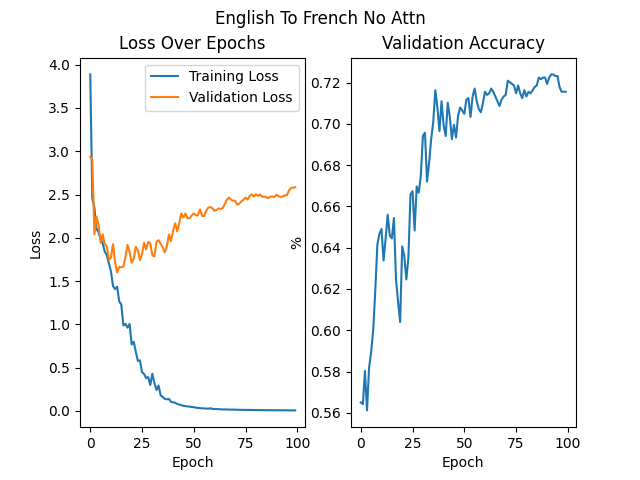
\includegraphics{plots/en2fr_noattn.png} &
%       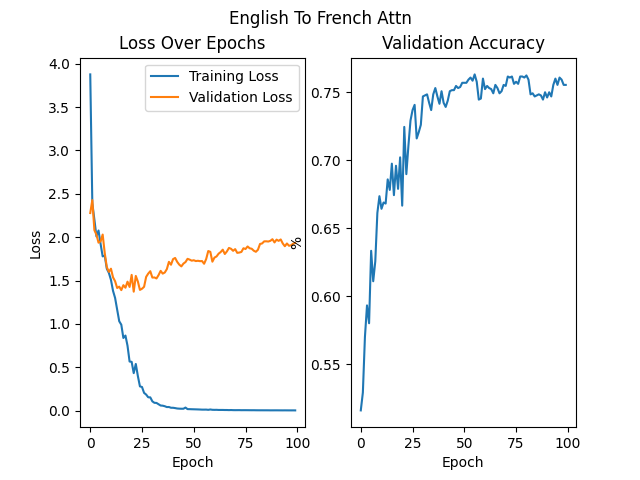
\includegraphics{plots/en2fr_attn.png} \\
%       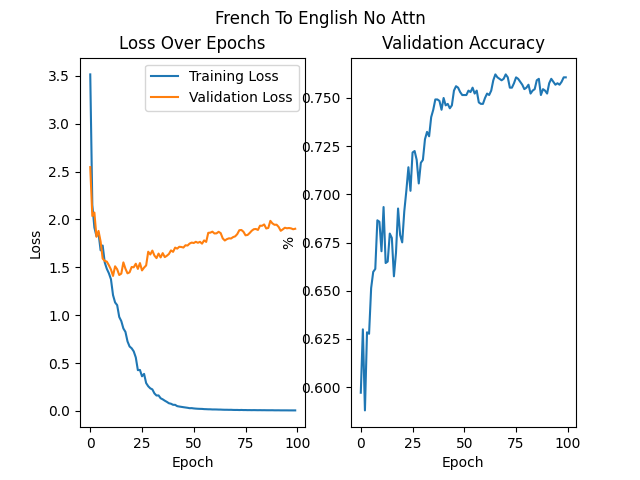
\includegraphics{plots/fr2en_noattn.png} &
%       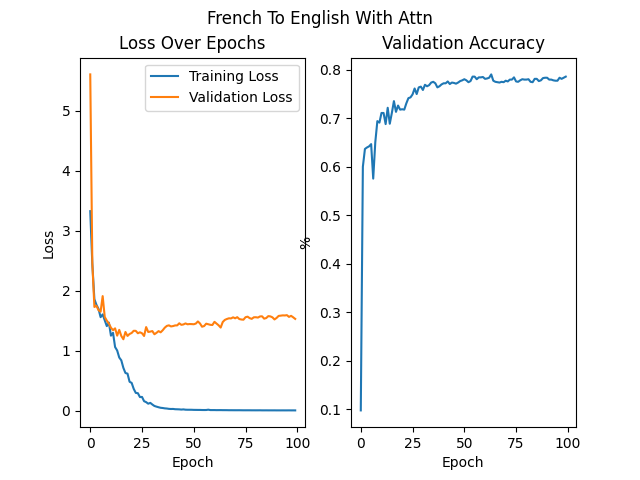
\includegraphics{plots/fr2en_attn.png} \\
%     \end{tabularx}
%     \caption{Training Curves}
%     \label{fig:losses}
% \end{figure}


% \section{Results}
% The models were evaluated on the test dataset in terms of
% accuracy on the sentence level and the word level. A
% sentence was considered correct if all the words in the
% sentence were translated correctly. A word was considered
% correct if the model output the exact word in the target
% language. A comparison in accuracy between the models with
% and without attention can be seen in Table
% \ref{tab:accuracy} below. 

% The models with attention outperformed the models without
% attention in both sentence and word level accuracy. Without
% attention, both translation tasks performed identically in
% sentence accuracy, whereas translating from French to
% English was slightly more accurate at the word level. This
% is mirrored when attention is added to the models.

% However, the English to French translation task benefitted
% much more from attention, and this is reflected by this task
% showing twice the sentence level accuracy as the French to
% English translation task.

% While the attention models performed well, all models still
% suffered from overfiting in the form of complete
% memorization of the training data. This is reflected in the
% sentences that the best performing model, the English to
% French Translator with attention, produced. For example, the
% model correctly translated the sentences: "He cooks dinner"
% and "He sings a song" because these sentences are in the
% training data but with 'He' replaced with 'She'. The model
% can only correctly translate sentences that are very similar
% to those found in the training set. 

% This is a limitation of
% the encoder-decoder architecture. Even with Badhanau
% attention, the model only uses one head of attention, and
% has no mechanism to allow the output tokens to update each
% other with context information. Additionally, there is no
% positional encoding present in the model. These issues
% compound the model's inability to understand the contextual
% meaning of each word in the input sequence and the output
% sequence. Finally, the training dataset only contains around
% 100 samples, which is not enough to train a model that can
% generalize well to unseen data.

% \begin{table}[h]
%     \begin{tabular}{|c|c|c|c|}
%         \hline
%         \multicolumn{4}{|c|}{\textbf{English $\rightarrow$ French}} \\
%         \hline
%         \hline
%         & \textbf{No Attention} & \textbf{With Attention} & \textbf{\% Difference} \\        
%         \hline
%         \textbf{Word Accuracy (\%)} & 71.56 & 76.83 & 7 \\
%         \hline
%         \textbf{Sentence Accuracy (\%)} & 1.83 & 12.84 & 602 \\
%         \hline
%         \multicolumn{4}{|c|}{\textbf{French $\rightarrow$ English}} \\
%         \hline
%         \hline
%         & \textbf{No Attention} & \textbf{With Attention} & \textbf{\% Difference} \\
%         \hline
%         \textbf{Word Accuracy (\%)} & 76.07 & 78.59 & 3 \\
%         \hline
%         \textbf{Sentence Accuracy (\%)} & 1.83 & 6.42 & 251 \\
%         \hline
%     \end{tabular}
%     \caption{Accuracy Results}
%     \label{tab:accuracy}
% \end{table}

\end{document}